\documentclass[12pt]{beamer}
\usepackage{../Estilos/BeamerMAF}
\usetheme{Warsaw}
\usecolortheme{crane}
%\useoutertheme{default}
\setbeamercovered{invisible}
% or whatever (possibly just delete it)
\setbeamertemplate{section in toc}[sections numbered]
\setbeamertemplate{subsection in toc}[subsections numbered]
\setbeamertemplate{subsection in toc}{\leavevmode\leftskip=3.2em\rlap{\hskip-2em\inserttocsectionnumber.\inserttocsubsectionnumber}\inserttocsubsection\par}
\setbeamercolor{section in toc}{fg=blue}
\setbeamercolor{subsection in toc}{fg=blue}
\setbeamercolor{frametitle}{fg=blue}
\setbeamertemplate{caption}[numbered]

\setbeamertemplate{footline}
\beamertemplatenavigationsymbolsempty
\setbeamertemplate{headline}{}


\makeatletter
\setbeamercolor{section in foot}{bg=gray!30, fg=black!90!orange}
\setbeamercolor{subsection in foot}{bg=blue!30}
\setbeamercolor{date in foot}{bg=black}
\setbeamertemplate{footline}
{
  \leavevmode%
  \hbox{%
  \begin{beamercolorbox}[wd=.333333\paperwidth,ht=2.25ex,dp=1ex,center]{section in foot}%
    \usebeamerfont{section in foot} \insertsection
  \end{beamercolorbox}%
  \begin{beamercolorbox}[wd=.333333\paperwidth,ht=2.25ex,dp=1ex,center]{subsection in foot}%
    \usebeamerfont{subsection in foot}  \insertsubsection
  \end{beamercolorbox}%
  \begin{beamercolorbox}[wd=.333333\paperwidth,ht=2.25ex,dp=1ex,right]{date in head/foot}%
    \usebeamerfont{date in head/foot} \insertshortdate{} \hspace*{2em}
    \insertframenumber{} / \inserttotalframenumber \hspace*{2ex} 
  \end{beamercolorbox}}%
  \vskip0pt%
}
\makeatother

\makeatletter
\patchcmd{\beamer@sectionintoc}{\vskip1.5em}{\vskip0.8em}{}{}
\makeatother

\newlength{\depthofsumsign}
\setlength{\depthofsumsign}{\depthof{$\sum$}}
\newcommand{\nsum}[1][1.4]{% only for \displaystyle
    \mathop{%
        \raisebox
            {-#1\depthofsumsign+1\depthofsumsign}
            {\scalebox
                {#1}
                {$\displaystyle\sum$}%
            }
    }
}
\def\scaleint#1{\vcenter{\hbox{\scaleto[3ex]{\displaystyle\int}{#1}}}}
\def\scaleoint#1{\vcenter{\hbox{\scaleto[3ex]{\displaystyle\oint}{#1}}}}
\def\bs{\mkern-12mu}


\date{22 de octubre de 2021}

\title{\large{La delta de Dirac}}
\subtitle{Previo al Tema 3}
\author{M. en C. Gustavo Contreras Mayén}

\begin{document}
\maketitle
\fontsize{14}{14}\selectfont
\spanishdecimal{.}

\section*{Contenido}
\frame{\tableofcontents[currentsection, hideallsubsections]}

\section{Introducción}
\frame{\tableofcontents[currentsection, hideothersubsections]}
\subsection{Dirac y la función \texorpdfstring{$\delta(t)$}{d(t)}}

\begin{frame}
    \frametitle{Orígenes de la función}
La función $\delta$ de Dirac es una función extraña pero útil que tiene muchas aplicaciones en ciencia, ingeniería y matemáticas. 
\end{frame}
\begin{frame}
\frametitle{Propuesta por Dirac}
La función $\delta$ fue propuesta en 1930 por Paul Dirac en el desarrollo del formalismo matemático de la mecánica cuántica. 
\\
\bigskip
\pause
Necesitaba una función que fuera cero en todas partes, excepto en un solo punto, donde era discontinua y se comportaba como un pico infinitamente alto e infinitamente estrecho de área unitaria.
\end{frame}    
\begin{frame}
\frametitle{Controversia por la función}
Los matemáticos se apresuraron a señalar que, estrictamente hablando, no hay ninguna función que tenga estas propiedades. 
\\
\bigskip
\pause
Pero Dirac supuso que sí, y procedió a utilizarlo con tanto éxito que se desarrolló una nueva rama de las matemáticas para justificar su uso.
\end{frame}
\begin{frame}
\frametitle{Nueva área de estudio}
Esta área de las matemáticas se denomina \emph{teoría de funciones generalizadas} y desarrolla, con todo detalle, la base de la función $\delta$ de Dirac.
\\
\bigskip
\pause
Este tratamiento riguroso es necesario para justificar el uso de estas funciones discontinuas, pero para el físico las interpretaciones físicas más simples son igualmente importantes.
\end{frame}

\section{Funciones singulares en física}
\frame{\tableofcontents[currentsection, hideothersubsections]}
\subsection{Utilidad en la física}

\begin{frame}
\frametitle{Casos ideales}
Las situaciones físicas se modelan generalmente mediante ecuaciones y operaciones sobre funciones continuas.
\\
\bigskip
\pause
A veces, sin embargo, es útil considerar idealizaciones discontinuas, como la densidad de masa de una masa puntual o la fuerza de un impulso mecánico infinitamente rápido.
\end{frame}
\begin{frame}
\frametitle{Funciones singulares}
Las funciones que describen estas ideas son obviamente extremadamente discontinuas, porque ellas y todas sus derivadas deben divergir.
\\
\bigskip
\pause
Por esta razón, a menudo se les llama \emph{funciones singulares}.
\end{frame}
\begin{frame}
\frametitle{Función $\delta(t)$ como función singular}
La función $\delta$ de Dirac se desarrolló para describir funciones que involucran este tipo de discontinuidades y proporcionar un método para manejarlas en ecuaciones que normalmente solo involucran funciones continuas.
\end{frame}

\subsection{El impulso ideal}

\begin{frame}
\frametitle{El impulso en mécanica}
A menudo, el primer encuentro de un estudiante de física con la función $\delta$ es el impulso \enquote{ideal}.
\\
\bigskip
\pause
En mecánica, un impulso es una fuerza que actúa sobre un objeto durante un período de tiempo finito.
\end{frame}
\begin{frame}
\frametitle{Gráfica de un impulso}
Considera la fuerza realista representada en la siguiente figura:
\pause
\begin{figure}[H]
    \centering
    \subfloat[]{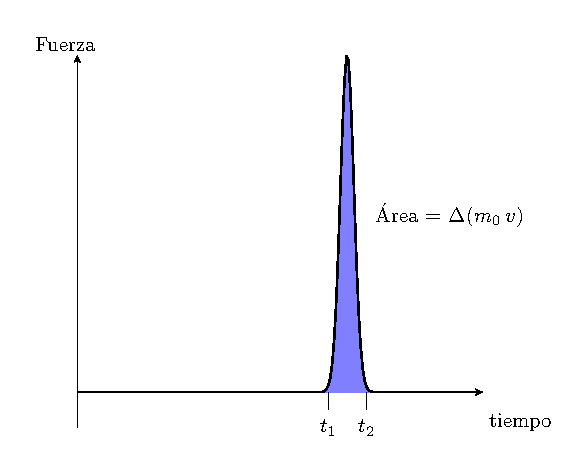
\includegraphics[width=0.5\textwidth]{Imagenes/delta_Dirac_Momento_00.eps}\label{fig:f1}}
    \subfloat[]{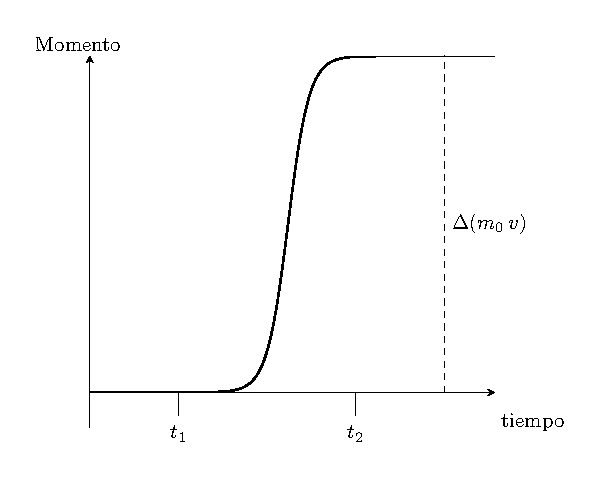
\includegraphics[width=0.5\textwidth]{Imagenes/delta_Dirac_Momento_01.eps}\label{fig:f2}}
    %\caption{Cambio en la fuerza y momento.}
\end{figure}
\end{frame}
\begin{frame}
\frametitle{Descripción del impulso}
Vale cero hasta $t = t_{1}$, cuando aumenta suavemente desde cero hasta su valor máximo, y luego finalmente regresa a cero en $t = t_{2}$.
\\
\bigskip
\pause
Cuando esta fuerza se aplica a un objeto de masa $m_{0}$, el momento en la dirección de la fuerza aplicada cambia, como se muestra en la figura (\ref{fig:f2}).
\end{frame}
\begin{frame}
\frametitle{Cambio en el momento}
\begin{figure}
    \centering
    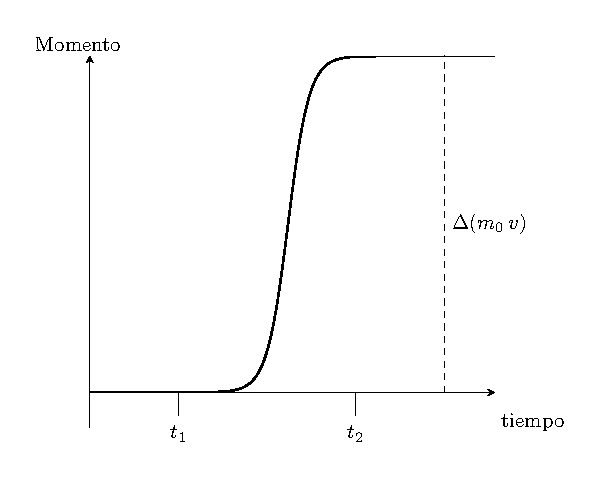
\includegraphics[scale=0.9]{Imagenes/delta_Dirac_Momento_01.eps}
\end{figure}

\end{frame}
\begin{frame}
\frametitle{Momento constante}
La cantidad de movimiento permanece constante hasta $t = t_{1}$, cuando comienza a cambiar continuamente hasta alcanzar su valor final en $t = t_{2}$.
\end{frame}
\begin{frame}
\frametitle{Momento constante}
El cambio neto en el momento $\Delta (m_{0} \, v)$ es igual al área debajo de la curva de la fuerza:
\pause
\begin{align}
\begin{aligned}[b]
\scaleint{5ex}_{\bs -\infty}^{\infty} F(t) \dd{t} &= \scaleint{5ex}_{\bs t_{1}}^{t_{2}} F(t) \dd{t} = \\[0.5em]
&= \scaleint{5ex}_{\bs t_{1}}^{t_{2}} m_{0} \dv{v}{t} \dd{t} = \\[0.5em]
&= m_{0} \, v \, \eval_{t_{2}} - m_{0} \, v \, \eval_{t_{1}} = \\[0.5em]
&= \Delta (m_{0} \, v) 
\end{aligned}
\label{eq:ecuacion_05_01}
\end{align}
\end{frame}
\begin{frame}
\frametitle{El impulso ideal}
Un impulso ideal genera todo su cambio de momento instantáneamente, en el único punto $t = t_{0}$, como se muestra en la figura:
\end{frame}
\begin{frame}
\frametitle{Cambio instantáneo en el momento}
\begin{figure}[H]
    \centering
\subfloat[]{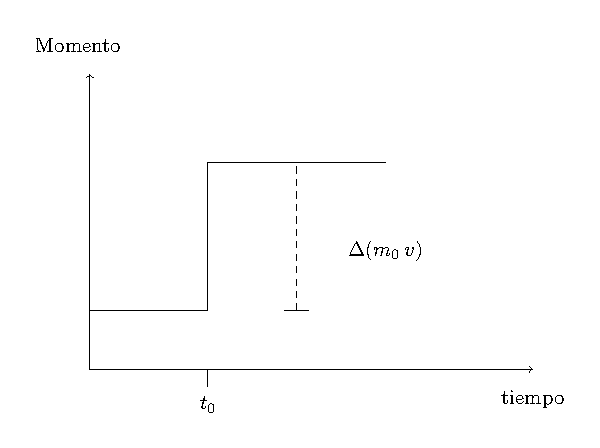
\includegraphics[width=0.5\textwidth]{Imagenes/delta_Dirac_Momento_02.eps}\label{fig:f2_1}}
\subfloat[]{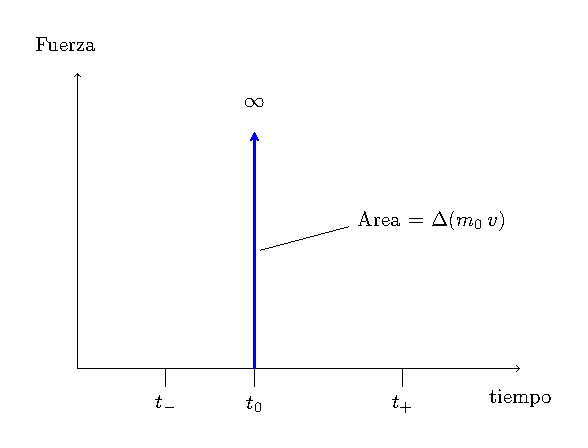
\includegraphics[width=0.5\textwidth]{Imagenes/delta_Dirac_Momento_03.eps}\label{fig:f2_2}}
%\caption{Cambio instantáneo en el momento.}
\end{figure}    
\end{frame}
\begin{frame}
\frametitle{Situación no tan real}
Por supuesto, que esto no es muy realista, ya que se requiere una fuerza infinita para cambiar el momento de una masa finita en un tiempo \enquote{cero}.
\\
\bigskip
\pause
Pero es un experimento mental aceptable, porque podríamos estar considerando el límite en el que un proceso físico ocurre más rápido de lo que cualquier medición puede detectar.
\end{frame}
\begin{frame}
\frametitle{Fuerza instantánea}
La fuerza de un impulso ideal no puede graficarse como función del tiempo en el sentido normal.
\\
\bigskip
\pause
La fuerza existe solo por un instante, y por lo tanto vale cero en todas partes, excepto en $t = t_{0}$, cuando es infinita. 
\end{frame}
\begin{frame}
\frametitle{Tipo de infinito}
Pero esto no es un infinito cualquiera.
\\
\bigskip
\pause
Dado que el cambio total de momento debe ser $\Delta (m_{0} \, v)$, la fuerza debe divergir para que su área bajo la curva cumpla (para todo $(t_{-} < t_{+})$:
\pause
\begin{align}
\scaleint{5ex}_{\bs t_{-}}^{t_{+}} F(t) \dd{t} = \begin{cases}
\Delta (m_{0} \, v) & t_{-} < t_{+} \\
0 & \mbox{en otro valor}
\end{cases}
\label{eq:ecuacion_05_02}
\end{align}
\end{frame}
\begin{frame}
\frametitle{Cambio en el momento}
En otras palabras, cualquier integral que incluya el punto $t_{0}$ da un cambio de momento de $\Delta (m_{0} \, v)$.
\\
\bigskip
\pause
Por otro lado, las integrales que excluyen a $t_{0}$ no deben dar ningún cambio de momento.
\end{frame}
\begin{frame}
\frametitle{Gráfica del impulso}
Graficamos esto simbólicamente como se muestra en la figura:
\begin{figure}
    \centering
    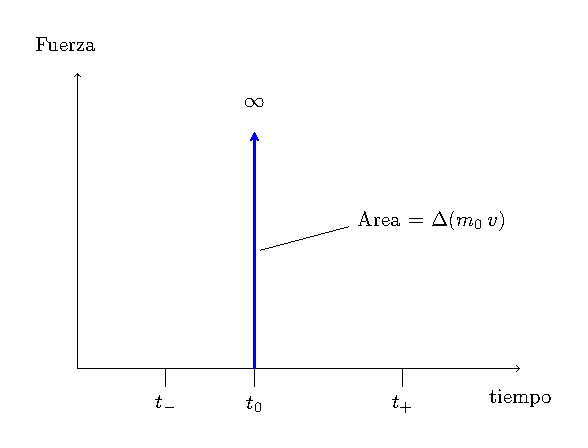
\includegraphics[scale=0.75]{Imagenes/delta_Dirac_Momento_03.eps}
\end{figure}
\end{frame}
\begin{frame}
\frametitle{Impulso infinito}
Un pico de ancho cero con una flecha indica que la función va al infinito, mientras que el área del impulso generalmente se indica mediante un comentario en el gráfico, como se muestra en la figura, o algunas veces por la altura de la flecha.
\end{frame}
\begin{frame}
\frametitle{Utilidad de la función delta}
La función $\delta$ de Dirac $\delta (t)$ fue diseñada para representar exactamente este tipo de función \enquote{patológica}.
\\
\bigskip
\pause
La $\delta (t)$ vale cero en todas partes, excepto en $t = 0$, cuando es infinito.
\end{frame}
\begin{frame}
\frametitle{Tipo especial de infinito}
De nuevo, esto no es cualquier infinito.
\\
\bigskip
\pause
Diverge de tal manera que cualquier integral que incluya $t = 0$ tiene el valor de $1$, es decir (para todo $t_{-} < t_{+}$):
\pause
\begin{align}
\int_{t_{-}}^{t_{+}} \delta (t) \dd{t} = \begin{cases}
1 & t_{-} < t_{+} \\
0 & \mbox{en otro valor}
\end{cases}
\label{eq:ecuacion_05_03}
\end{align}
\end{frame}
\begin{frame}
\frametitle{Gráfica de la función delta}
De manera simbólica la gráfica de la función $\delta (t)$ se muestra en la figura:
\pause
\begin{figure}[H]
        \centering
        \includegraphics[scale=1]{Imagenes/delta_Dirac_Momento_05.eps}
        % \caption{La función delta de Dirac $\delta (t)$}
        % \label{fig:figura_05_03}
    \end{figure}
\end{frame}
\begin{frame}
\frametitle{El impulso ideal}
El impulso ideal, discutido previamente, puede expresarse en términos de la función delta de Dirac desplazada:
\pause
\begin{align}
F(t) = \Delta (m_{0} \, v) \, \delta (t - t_{0})
\label{eq:ecuacion_05_04}
\end{align}
\pause
El argumento $t - t_{0}$ simplemente traduce el pico de la función para que ocurra en $t_{0}$ en lugar de $0$.
\end{frame}

\subsection{Masas y cargas puntuales}

\begin{frame}
\frametitle{Representando cantidades}
En la física a menudo las ecuaciones involucran la masa por unidad de volumen $\rho_{m} (\va{r})$ en una región del espacio.
\\
\bigskip
\pause
Normalmente, $\rho_{m} (\va{r})$ es una función continua de posición, pero con la función $\delta$, también puede representar masas puntuales.
\end{frame}
\begin{frame}
\frametitle{Una masa puntual}
Una masa puntual tiene una cantidad finita de masa dentro de un solo punto del espacio, por lo que la densidad debe ser infinita en ese punto y cero en cualquier otro lugar.
\end{frame}
\begin{frame}
\frametitle{Recuperando la masa total}
Integrando la densidad de masa en un volumen $V$, se obtiene la masa total contenida:
\pause
\begin{align}
    \scaleint{5ex}_{\bs V} \rho_{m} (\va{r}) \dd{\tau} = \mbox{ masa total dentro de } V
    \label{eq:ecuacion_05_05}
    \end{align}
\end{frame}
\begin{frame}
\frametitle{Masa puntual}
Así, si hay un solo punto de masa $m_{0}$, ubicado en el origen, como se muestra en la figura:
\pause
\begin{figure}[H]
    \centering
    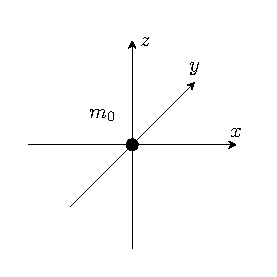
\includegraphics[scale=1.3]{Imagenes/delta_Dirac_Masa_Puntual.eps}
    %\caption{Una masa puntual en el origen.}
    \label{fig:figura_05_04}
\end{figure}
\end{frame}
\begin{frame}
\frametitle{Integral con el origen incluido}
Cualquier integral de volumen que incluya el origen debe dar la masa total como $m_{0}$, las integrales que excluyen el origen deben devolver cero. 
\end{frame}
\begin{frame}
\frametitle{Matemáticamente hablando}
En términos matemáticos:
\pause
\begin{align}
\scaleint{5ex}_{\bs V} \rho_{m} (\va{r}) \dd{\tau} = \begin{cases}
m_{0} & \mbox{origen incluido en } V \\
0 & \mbox{origen excluido en } V
\end{cases}
\label{eq:ecuacion_05_06}
\end{align}
\end{frame}
\begin{frame}
\frametitle{Función de densidad de masa}
Usando la función $\delta$ de Dirac, la función densidad de masa es:
\pause
\begin{align}
\rho_{m} (\va{r}) = m_{0} \, \delta(x) \, \delta(y) \, \delta(z)
\label{eq:ecuacion_05_07}
\end{align}
\end{frame}
\begin{frame}
\frametitle{Comprobando la integral}
La ec. (\ref{eq:ecuacion_05_06}) se puede verificar fácilmente expandiendo la integral como:
\pause
\begin{align}
\scaleint{5ex}_{\bs V} \rho_{m} (\va{r}) \dd{\tau} = \scaleiiint{5ex} m_{0} \, \delta(x) \, \delta(y) \, \delta(z) \dd{x} \dd{y} \dd{z}
\label{eq:ecuacion_05_08}
\end{align}
\end{frame}
\begin{frame}
\frametitle{Resultado de la integral triple}
Aplicar la ec. (\ref{eq:ecuacion_05_03}) a las tres integrales independientes devuelve $m_{0}$, solo cuando $V$ incluye el origen.
\end{frame}
\begin{frame}
\frametitle{Resultado de la integral triple}
Si en lugar del origen, la masa puntual está ubicada en el punto $(x_{0}, y_{0}, z_{0})$, se utilizan argumentos desplazados en cada una de las funciones $\delta$:
\pause
\begin{align}
\rho_{m} (\va{r}) = m_{0} \, \delta (x - x_{0}) \, \delta (y - y_{0}) \, \delta (z - z_{0})
\label{eq:ecuacion_05_09}
\end{align}
\end{frame}

\section{Dos definiciones de \texorpdfstring{$\delta (t)$}{d(t)}}
\frame{\tableofcontents[currentsection, hideothersubsections]}
\subsection{La \texorpdfstring{$\delta(t)$}{d(t)} como función generalizada}

\begin{frame}
\frametitle{Definiendo la función delta}
Hay dos formas comunes de definir la función $\delta$ de Dirac. 
\setbeamercolor{item projected}{bg=blue!70!black,fg=yellow}
\setbeamertemplate{enumerate items}[circle]
\begin{enumerate}[<+->]
\item El enfoque más riguroso, desde \emph{la teoría de funciones generalizadas}, lo define por su comportamiento dentro de las operaciones integrales.
\par
De hecho, nunca se supone que la función $\delta$ exista fuera de una integral.
\seti 
\end{enumerate}
\end{frame}
\begin{frame}
\frametitle{Definiendo la función delta}
En general, en ciencia e ingeniería se un poco más laxos y usan una segunda definición.
\setbeamercolor{item projected}{bg=blue!70!black,fg=yellow}
\setbeamertemplate{enumerate items}[circle]
\begin{enumerate}[<+->]
\conti
\item A menudo definen la función $\delta$ como \emph{el límite de una secuencia infinita de funciones continuas}.
\end{enumerate}
\end{frame}
\begin{frame}
\frametitle{Definiendo la función delta}
Además, como se demostró en los dos ejemplos anteriores, con frecuencia manipulan la función $\delta$ fuera de las integrales.
\pause
Por lo general, no hay problemas con este enfoque menos riguroso.
\end{frame}

\subsection{La \texorpdfstring{$\delta(t)$}{d(t)} como límite de una secuencia}

\begin{frame}
\frametitle{La función delta como límite}
La función $\delta$ puede verse como el límite de una secuencia de funciones, es decir:
\pause
\begin{align}
\delta(t) = \lim_{n \to \infty} \delta_{n} (t)
\label{eq:ecuacion_05_10}
\end{align}
donde $\delta_{n}(t)$ es finito para todos los valores de $t$.
\end{frame}
\begin{frame}
\frametitle{Tipos de secuencias}
Hay muchas secuencias de funciones que se acercan a la función $\delta$ de Dirac de esta manera. La más simple es la secuencia de función cuadrada definida por:
\begin{align}
\delta_{n} (t) = \begin{cases}
n & -\dfrac{1}{2 \, n} < t < \dfrac{1}{2 \, n} \\
0 & \mbox{en cualquier otro punto}
\end{cases}
\label{eq:ecuacion_05_11}
\end{align}
\end{frame}
\begin{frame}
\frametitle{Gráfica de la secuencia}
Como se muestra en la figura:
\begin{figure}[H]
    \centering
    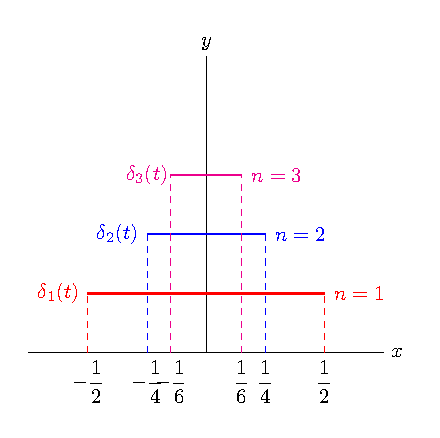
\includegraphics[scale=0.9]{Imagenes/plot_secuencia_delta_02.eps}
    % \caption{Primeras tres funciones de la secuencia.}
    % \label{fig:figura_05_06}
\end{figure}
\end{frame}
\begin{frame}
\frametitle{El área debajo de la curva}
Es claro que para cualquier valor de $n$:
\pause
\begin{align}
\scaleint{5ex}_{\bs -\infty}^{\infty} \delta_{n} (t) \dd{t} = 1
\label{eq:ecuacion_05_12}
\end{align}
en el límite cuando $n \to \infty$, $\delta_{n}(t) = 0$ para todo valor de $t$, excepto $t = 0$. 
\end{frame}
\begin{frame}
\frametitle{Otras secuencias delta}
Hay otras tres secuencias de funciones comunes que se acercan a la función $\delta$ de Dirac: las secuencias de:
\setbeamercolor{item projected}{bg=blue!70!black,fg=yellow}
\setbeamertemplate{enumerate items}[circle]
\begin{enumerate}[<+->]
\item Resonancia.
\item Gaussiana.
\item Sinc al cuadrado.
\end{enumerate}
\end{frame}
\begin{frame}
\frametitle{Otras secuencias delta}
Que se describen matemáticamente mediante:
\pause
\begin{align}
\begin{aligned}
\mbox{Resonancia:} \hspace{1cm} \delta_{n}(t) &= \dfrac{n/\pi}{1 + n^{2} \, t^{2}} \\[1em]
\mbox{Gaussiana:} \hspace{1cm} \delta_{n}(t) &= \dfrac{n}{\sqrt{\pi}} \, e^{-n^{2} t^{2}} \\[1em]
\mbox{Sinc cuadrada:} \hspace{1cm} \delta_{n}(t) &= \dfrac{\sin^{2} n \, t}{n \, \pi \, t^{2}} 
\end{aligned}
\label{eq:ecuacion_05_13}
\end{align}
\end{frame}
\begin{frame}
\frametitle{Secuencia delta para la función resonancia}
\begin{figure}[H]
    \centering
    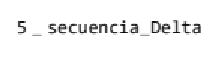
\includegraphics[scale=1]{Imagenes/secuencia_Delta_05.eps}
%     \caption{Gráfica de la secuencia delta para la función resonancia.}
%     \label{fig:figura_05_07}
\end{figure}
\end{frame}
\begin{frame}
\frametitle{secuencia delta para la función Gaussiana}
\begin{figure}[H]
    \centering
    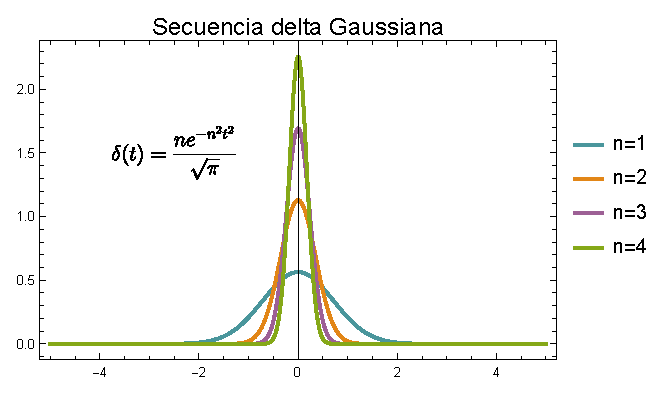
\includegraphics[scale=1]{Imagenes/secuencia_Delta_06.eps}
%     \caption{Gráfica de la secuencia delta para la función Gaussiana.}
%     \label{fig:figura_05_08}
\end{figure}
\end{frame}
\begin{frame}
\frametitle{secuencia delta para la función sinc al cuadrado}
\begin{figure}[H]
    \centering
    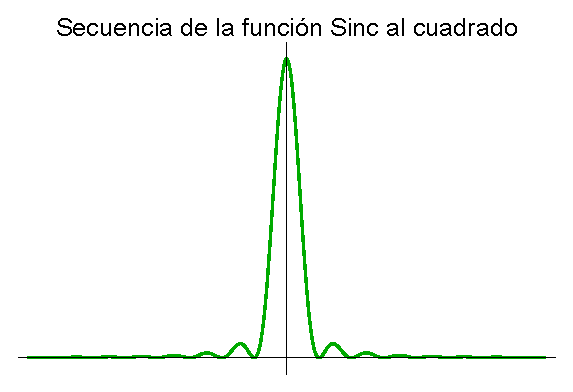
\includegraphics[scale=1]{Imagenes/secuencia_Delta_07.eps}
%     \caption{Gráfica de la secuencia delta para la función sinc al cuadrado.}
%     \label{fig:figura_05_09}
\end{figure}
\end{frame}
\begin{frame}
\frametitle{Área debajo de la curva}
Cada una de esas funciones tiene un área unitaria para cualquier valor de $n$, y es fácil calcularla cuando en el límite $n \to \infty$, $\delta_{n} (t) = 0$ para todo $t \neq 0$.
\end{frame}


\section{La \texorpdfstring{$\delta(t)$}{d(t)} por operaciones integrales}
\frame{\tableofcontents[currentsection, hideothersubsections]}
\subsection{Propiedad de la \texorpdfstring{$\delta(t)$}{d(t)}}

\begin{frame}
\frametitle{Matemáticamente hablando}
En matemáticas, la función $\delta$ se define por cómo se comporta dentro de una integral.
\\
\bigskip
\pause
Cualquier función que se comporte como $\delta (t)$ en la siguiente ecuación es por definición una función $\delta$:
\pause
\begin{align}
\scaleint{5ex}_{\bs t_{-}}^{t_{+}} f(t) \, \delta(t {-} t_{0}) \dd{t} = \begin{cases}
f(t_{0}) & t_{-} < t_{0}  < t_{+} \\
0 & \mbox{en otros puntos}
\end{cases}
\label{eq:ecuacion_05_14}
\end{align}
\end{frame}
\begin{frame}
\frametitle{Matemáticamente hablando}
\begin{align*}
\scaleint{5ex}_{\bs t_{-}}^{t_{+}} f(t) \, \delta(t - t_{0}) \dd{t} = \begin{cases}
f(t_{0}) & t_{-} < t_{0}  < t_{+} \\
0 & \mbox{en otros puntos}
\end{cases}
\end{align*}        
donde $t_{-} < t_{+}$ y $f (t)$ es cualquier función continua de buen comportamiento.
\\
\bigskip
\pause
Esta operación a veces se denomina \emph{integral de filtrado}, porque selecciona el valor único $f(t_{0})$ de $f(t)$.
\end{frame}
\begin{frame}
\frametitle{La integral de filtrado}
Debido a que esta es una definición, no es necesario probarla, pero se debe demostrar su coherencia con nuestra definición anterior y las aplicaciones de la función.
\end{frame}
\begin{frame}
\frametitle{La integral de filtrado}
Si $t_{-} < t_{0}  < t_{+}$, el rango de la integral se puede cambiar para que sea una región infinitesimal de tamaño $2 \, \varepsilon$ centrada alrededor de $t_{0}$, sin cambiar el valor de la integral.
\end{frame}
\begin{frame}
\frametitle{La integral de filtrado}
Esto es cierto porque $\delta (t - t_{0})$ se anula en todas partes excepto en $t = t_{0}$. Esto es:
\pause
\begin{align}
\scaleint{5ex}_{\bs t_{-}}^{t_{+}} f(t) \, \delta (t - t_{0}) \dd{t} = \scaleint{5ex}_{\bs t_{-} - \varepsilon}^{t_{+} + \varepsilon} f(t) \, \delta (t - t_{0}) \dd{t} 
\label{eq:ecuacion_05_15}
\end{align}
\end{frame}
\begin{frame}
\frametitle{Aprovechando la continuidad}
Como $f (t)$ es una función continua, sobre la región infinitesimal es efectivamente una constante, con valor $f(t_{0})$. Por lo tanto:
\pause
\begin{align}
\begin{aligned}[b]
\scaleint{5ex}_{\bs t_{-}}^{t_{+}} f(t) \, \delta (t - t_{0}) \dd{t} &= f(t_{0}) \, \scaleint{5ex}_{\bs t_{-} - \varepsilon}^{t_{+} + \varepsilon} \delta (t - t_{0}) \dd{t} \\[0.5em]
&= f(t_{0})
\end{aligned}
\label{eq:ecuacion_05_16}
\end{align}
\end{frame}
\begin{frame}
\frametitle{Valor de la integral}
Esto \enquote{demuestra} la primera parte de la ec. (\ref{eq:ecuacion_05_14}).
\\
\bigskip
\pause
La segunda parte, cuando $t_{0}$  no está dentro del rango $t_{-} < t_{0}  < t_{+}$, se sigue fácilmente porque, en este caso, $\delta (t - t_{0})$ es cero para todo el rango del integrando.
\end{frame}
\begin{frame}
\frametitle{Representación de la integral de filtrado}
La siguiente figura muestra una representación de la integración en la ec. (\ref{eq:ecuacion_05_14}).
\\
\bigskip
\pause
El integrando es un producto de una función de $\delta$ desplazada y la función continua $f (t)$.
\end{frame}
\begin{frame}
\frametitle{La función $f(t)$ y la $\delta(t)$}
\begin{figure}
    \centering
    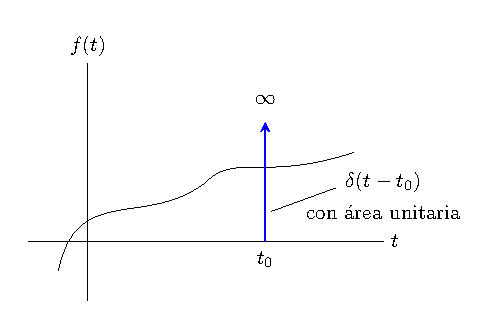
\includegraphics[scale=1]{Imagenes/plot_propiedad_desplazamiento_02.eps}
\end{figure}
\end{frame}
\begin{frame}
\frametitle{Usando el valor de la delta}
Debido a que la función $\delta$ es cero en todas partes excepto en $t = t_{0}$, el integrando va a una función $\delta$ ubicada en $t = t_{0}$, con un área escalada por el valor de $f (t_{0})$.
\end{frame}
\begin{frame}
\frametitle{Resultado de la integral de filtrado}
\begin{figure}[H]
    \centering
    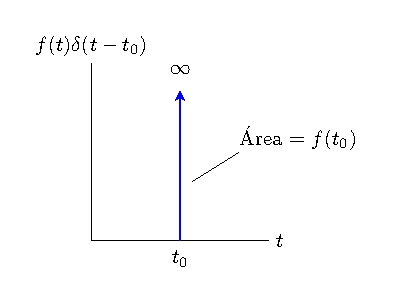
\includegraphics[scale=1]{Imagenes/plot_propiedad_desplazamiento_03.eps}
\end{figure}
\end{frame}
\end{document}